\chapter{Results}


\section{Repositories for Code Management}

A GitHub organization is created to manage all repositories related to the project. Within this organization, four main repositories essential for the project were maintained:
\begin{itemize}
    \item \verb|digital_twin|: Stored all the code and related documentation for the digital twin model.
    \item \verb|report|: Contained the technical report of the project.
    \item \verb|serial_motor|: Held the nodes responsible for executing the model and motor control.
    \item \verb|ros_arduino_bridge|: Included the Arduino Mega scripts required for the project.
\end{itemize}

\section{Build a workspace with colcon}

On both machines, a designated workspace is created for the project. To create a workspace within the ROS2 ecosystem the standard build toll colcon must be installed. Colcon simplifies the process of building, testing, and packaging multiple interdependent ROS 2 packages in a single workspace. To create the workspaces the "ROS2 Rolling Beginner: Client libraries tutorial" is followed.\autocite{openroboticsUsingColconBuild} Additionally a CMake configuration file and an XML metadata file were generated. 

The CMakeLists.txt file defines the build configuration, such as source files, dependencies, and build targets, while the package.xml file provides metadata about the package, including its name, version, authors, and dependencies. Together, these files enable colcon to properly build and integrate the packages into the workspace. \autocite{dirkUniversalBuildTool}

\section{Build of prototype robot}

The starting point of the project is the building part of the real-world robot. The initial idea is to create a custom-made robot. This robot is designed with a body measuring 50x50x20 cm and equipped with four wheels, with the two back wheels motor-controlled. For the body 3D printed material is used. 
The architecture and control system were inspired by a previous project, in which the control system of the farmbot system is used to control the robot. The robot's case is successfully built, however the connection to the motors from the motor controller where more complicated than predicted.  

To streamline the initial stages of the project, the prototype is built using the base of an existing robot system. This recycled robot provided a simple and practical starting point, as it minimized the time and effort required for fabrication and assembly. The design features a three-wheel configuration, with two powered wheels at the back and a single wheel at the front for support and steering. Since this base structure is taking over from an existing robot, the project changed the initial robot design to a three-wheel configuration. The case is made of a transparent plexiglass plate measuring 21.5 x 10.5 x 0.3 cm.  

Two power sources, in the form of battery-stacks, are mounted on the case: one dedicated to powering the motors and the other supplying power to the Raspberry Pi. A motor\-driver is used to convert the high voltage from the power station into a smaller voltage suitable for controlling the motors. This is managed by an Arduino Mega in this project. To conserve energy, an on/off switch is integrate. 
This is soldered to the existing electrical cables of the motor driver, ensuring a secure and efficient connection. This switch exclusively turns the power station on and off. It extends the existing switch, which manages the flow of electricity between the motor driver and the motor controller. The onboard computer is a Raspberry Pi 4 running the robot control system ROS2 Rolling. To power the Raspberry Pi 4, a Dexter GoPiGo3 head is used as a bridge to connect to the power station. Serial communication over USB connects the onboard computer to the motor controller. The robot's movement is initially established using the FarmBot software.

\begin{figure}[h]
    \centering
    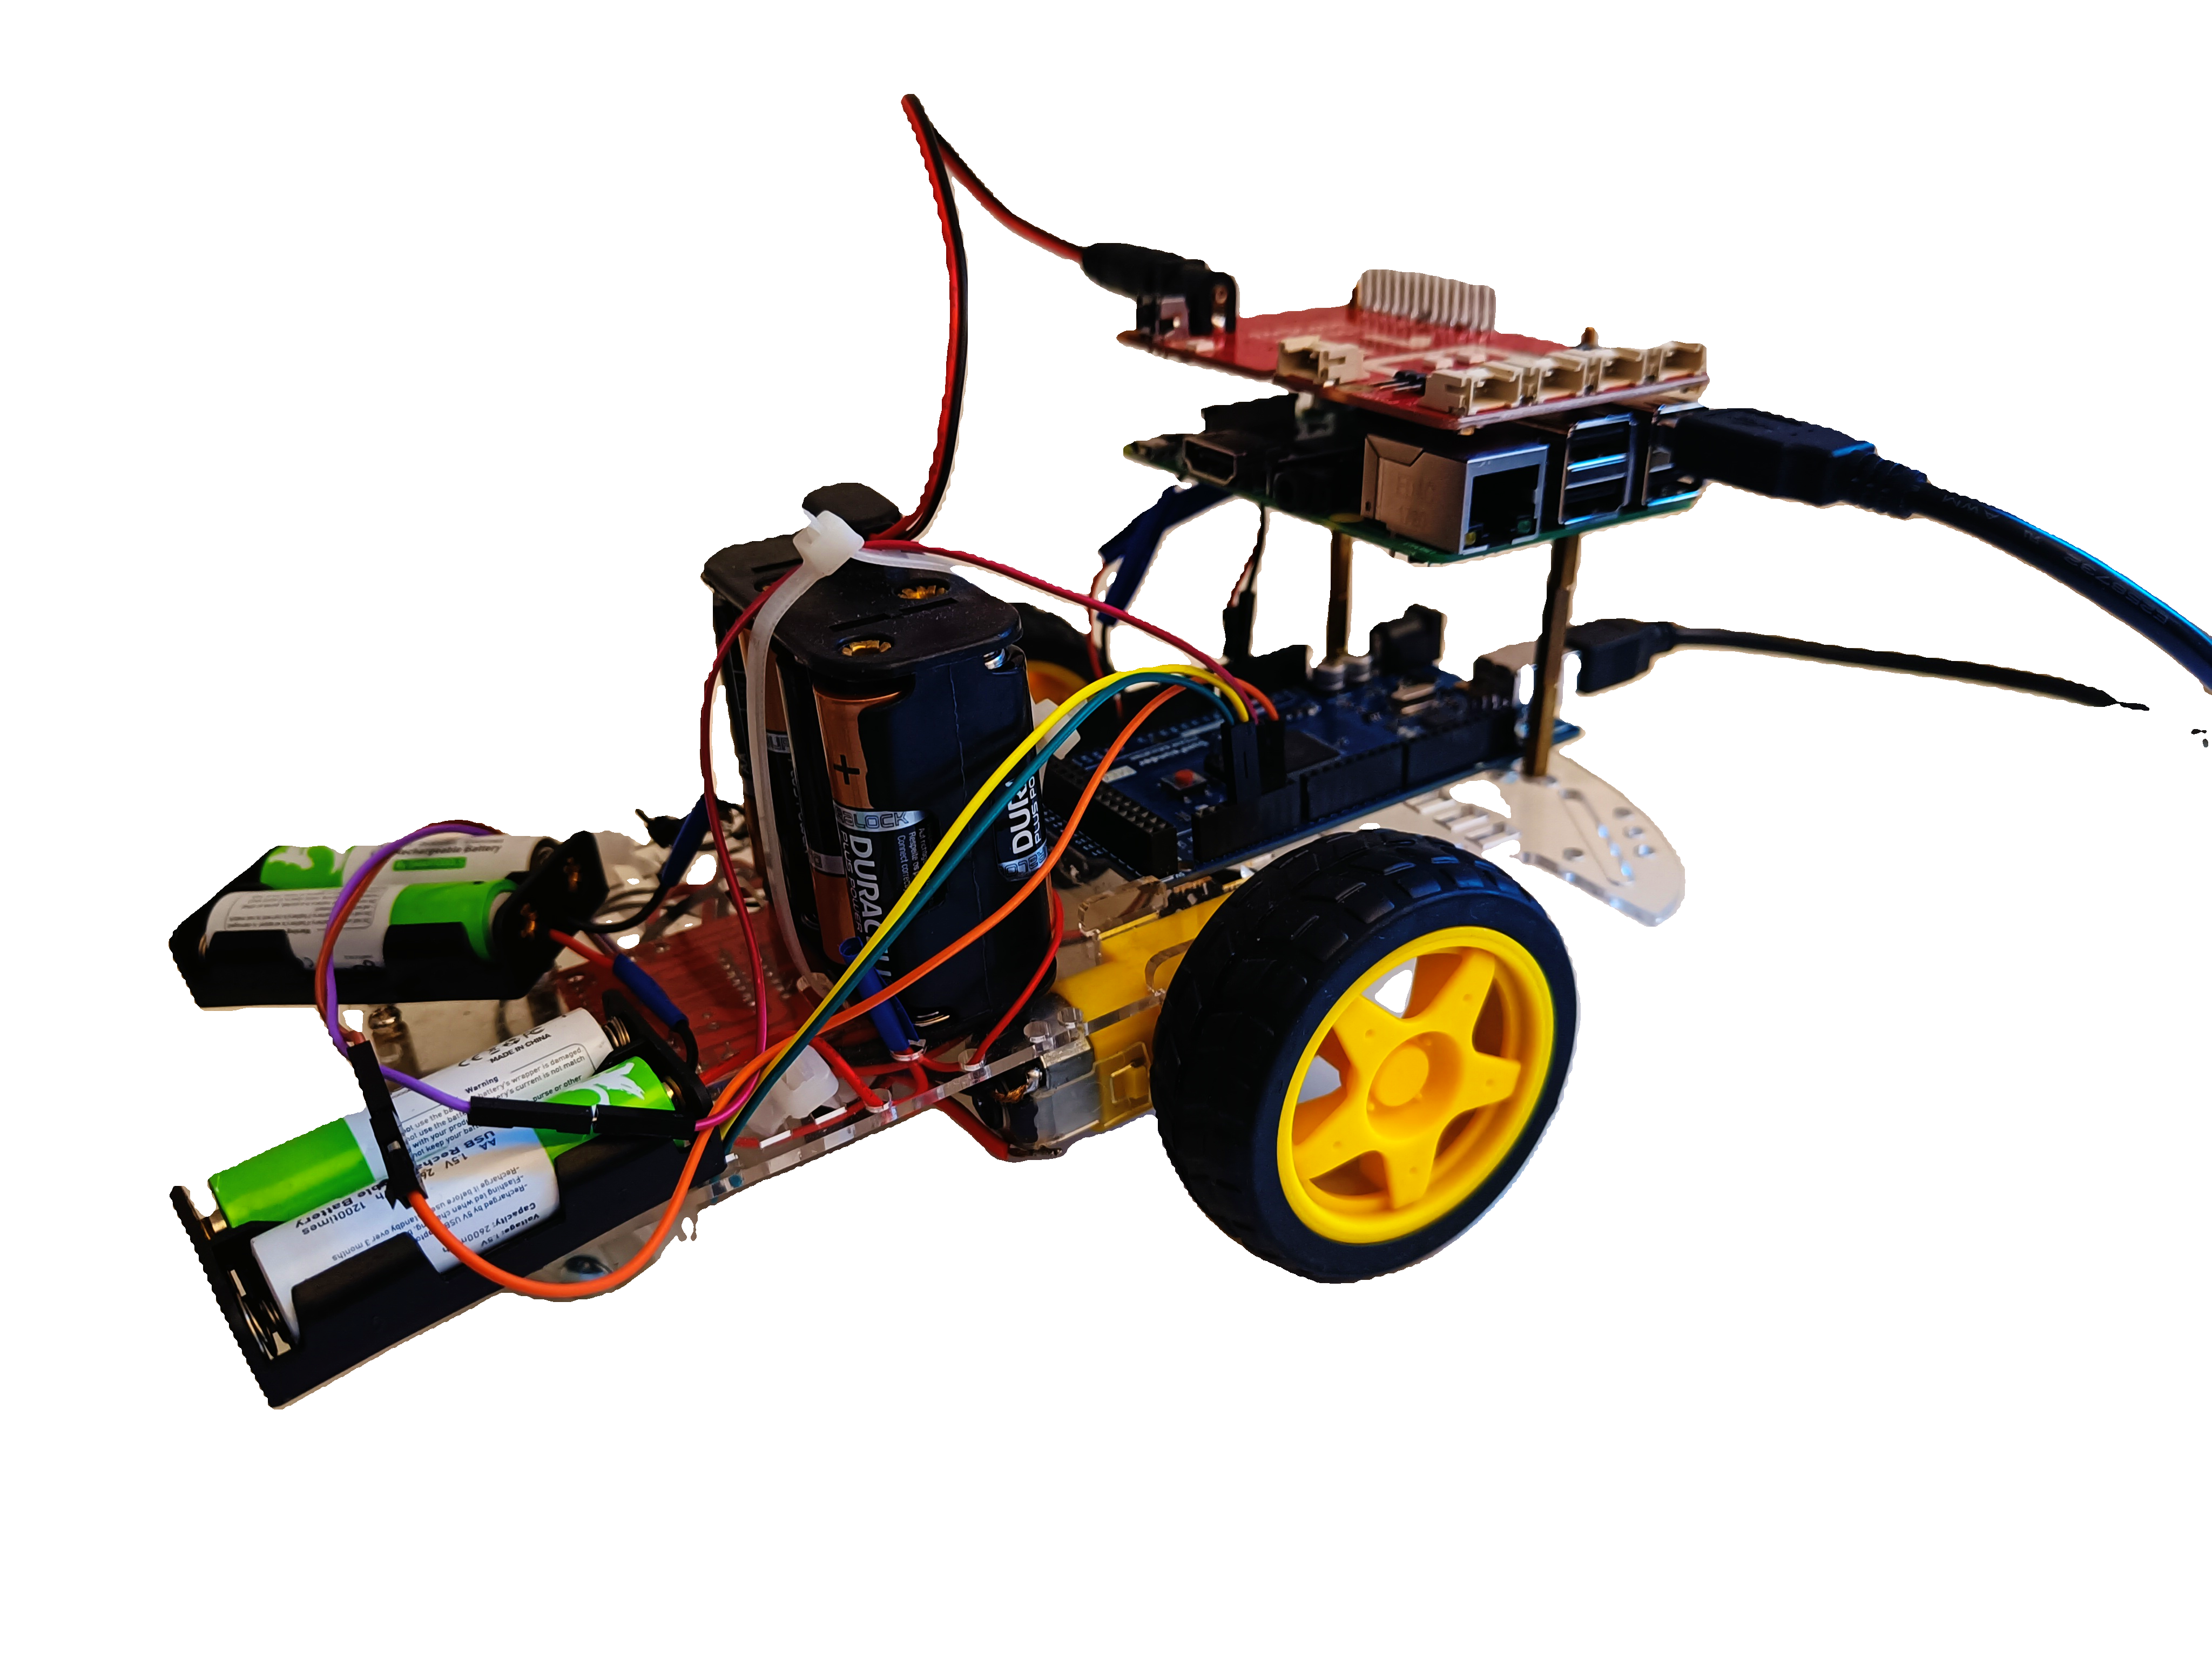
\includegraphics[width=0.7\textwidth]{Figures/Batmoblie.PNG}
    \caption{Prototype ``Batmobile''}

\end{figure}

\section{Installation hardware and software}


The ROS2 ecosystem operates most effectively on a Linux-based system; therefore, a virtual machine with Ubuntu 24.04 is configured using VirtualBox to provide access to such an environment. This approach is efficient for the first steps of the project. The two tools Rviz2 and Gazebo could be successfully started. Further, the first URDF file of this project is developed within the virtual machine and thereby primarily displayed in the two tools Rviz2 and Gazebo within the virtual machine. The installation of Gazebo initially presented challenges due to incorrect configuration settings, which are explained in detail in the following Gazebo section.
The For the further development of the project, the use of the virtual machine created significant challenges, primarily related to establishing a reliable connection between the control unit and the edge device. To address this issue, an attempt is made to connect the control device directly to the network using an Ethernet cable to reduce potential network conflicts. Even though the connection between the two machines could not be established.
An alternative approach involved installing a full Ubuntu terminal environment. This Windows-specific solution requires downloading the Ubuntu 24.04 terminal from the Microsoft Store. Windows 10 and 11 include the Windows Subsystem for Linux (WSL2), a compatibility layer designed to run a Linux environment seamlessly within the Windows operating system \autocite{microsoftWasIstWindowsSubsystem2023}.
The control machine is connected to the network via an Ethernet cable. While this setup enabled a one-way connection from the control unit to the edge device, the reverse connection remained unsuccessful.
The third attempt is to use Docker containers, this approach is a widely used in the industry and has the benefit of running the ecosystem in a separate container. Although a connection between the two containers is successfully established, the installation of Gazebo and the visualization of the robot model failed within this setup.
As a result, the control unit is reconfigured with a full installation of the Ubuntu 24.04 operating system, allowing for a fresh and stable environment.  The detailed rebooting process can be found in the installation guide A1, placed in the appendix. 
ROS2 Rolling is successfully installed on both machines, and communication between them is verified using the demo nodes talker and listener. The connection setup involved configuring the ROS DOMAIN ID to 0 and specifying the ROS IP for both machines in their respective .bashrc files. Additionally, the command source "/opt/ros/rolling/setup.bash" is added to the .bashrc files to ensure the ROS setup file is automatically sourced in every new shell session, eliminating the need for manual sourcing.

\subsection{Network configuration}

At home, both devices were successfully connected to the local Wi-Fi, allowing seamless communication between them. However, this setup is not successful in the ZHAW environment.
Due to the network configurations at ZHAW, the Raspberry Pi 4 is connected to the IoT network, while the control device is linked to the student network. Communication between these two networks is possible but restricted. To enable communication between two nodes via ROS 2 topics, both nodes must either reside within the same network or be accessible across connected networks. A solution to address the network limitations could not be identified within the available timeframe. Therefore, the ZHAW network is not used within the scope of this project. 


%% CG: NEW SECTION: "Building the digital twin"

%% CG: This section requires how the digital twin handles and responds to incoming messages. Somehow, I am missing 
%% this information.

\section{Develop URDF file}

The development of the first URDF file (batmobile.urdf) is early established in the project. The guide of the ROS2 Rolling tutorials of the official website and the Articubot one tutorials were followed to develop the URDF file. The batmobile.urdf file is written with the Xacro program, but the structure of the parent file and child file is not used. At the top of the script, the XML version and name of the project were defined. The second section contained information on the material colour. It specified the colour codes which were used to display a specific colour. After the definition of the material colours, the main section started. This section contained links and joints, which describe the robot's visual appearance. Each robot part is represented as a link and each connection between two parts as a joint.
In the course of the project, the structure of the URDF file underwent significant modifications. The final URDF file followed the parent-child structure,  which is refined based on insights gained through iterative experimentation.
The final setup consisted of one parent file and three child files, each serving a specific purpose.
The parent file managed the inclusion of child files and organized the overall structure of the robot description. Each child file is included using the <xacro:include> tag.
The three child files were the following: 
\verb|core_model.xacro| : Contained the constants for the robot's dimensions, as well as the joints and links which describe the robot's physics. The file structure of the \verb|diffbot_description.urdf.xacro|  from the \verb|ROS2_control_demos|  repository is used to build this file \autocite{frohlichROS2\_control\_demosROS2_control\_demo\_descriptionDiffbot}.
\verb|materials.xacro| : Contained the colour codes. 
\verb|gz_control.xacro|: Contained the Differential Drive Plugin. The Gazebo plugin is used to control and simulate the movement of a robot with a differential drive system. A differential drive system is a type of robot locomotion where two wheels, typically located on either side of the robot, are independently controlled to move the robot forward, backwards, and to rotate around its centre \autocite{riveraUnmannedGroundVehicle2019}.

\section{Visualization with Rviz2}

For the first attempt to launch the model in Rviz2 the shell commands were used: 

\lstinputlisting[caption={shell commands to run Rviz2}, label={lst:Rviz2}]{Code/rviz_shell.bash}

Over the course of the project, a launch file is established to publish the URDF data under the robot description in RViz, further, the GUI State Publisher is enabled, allowing for interactive movement of the robot's wheels. The primary model which is shown in the figure~\ref{fig:primary_model}, contained two wheel arms, which hold the front wheel. This construction is visually closer to the real robot but hinders the free movement of the front wheel in the model. Therefore the second model used a box element to fill the space the arms would be placed in and used a sphere instead of a cylinder element to model the front wheel, as seen in the figure~\ref{fig:second_model}. The first two models were able to display the joint movement when using the gui stat publisher panel, but the model's body is static and could not move from one point to another.


\begin{figure}[h]
    \centering
    \includegraphics[width=0.7\textwidth]{Figures/fir_side.png}
    \caption{Primary Model}
    \label{fig:primary_model}
\end{figure}

\begin{figure}[h]
    \centering
    \includegraphics[width=0.7\textwidth]{Figures/sec_side.png}
    \caption{Second Model}
    \label{fig:second_model}
\end{figure}

\clearpage

In the final model, the additional link \verb|dummy_link| is added to generate a world-like layer. The idea is to vizualize a world component which could be used as a fix point on which the model could be placed and move around. This idea is then implemented, with in the gazebo simulation, but not further followed for the Rviz2 model. The final tf2 tree structure is shown in the figure~\ref{fig:tf_tree}.

\begin{figure}
    \centering
    \includegraphics[width=0.7\textwidth]{Figures/frames_2024-12-08_22.48.01.pdf}
    \caption{tf2 tree structure}
    \label{fig:tf_tree}

\end{figure}

\begin{figure}
    \centering
    \includegraphics[width=0.7\textwidth]{Figures/final_model.png}
    \caption{Final Model}

\end{figure}


\clearpage

\section{Gazebo}

%% CG: No past tense! Please state how you installed GAZEBO and what you found out for choosing the correct version!
%% THis paragraph is missing references. 
The Gazebo simulator is successfully installed and launched. However, initial attempts to use the simulator fail due to the installation of an outdated version. The simulator is initially installed using the default method, which installs Gazebo Harmonic. Since compatibility between the ROS2 distribution and the Gazebo version is critical, Gazebo Ionic is installed to resolve the issue. The detailed installation prozess can be faund in the installation guide A3. 
Early attempts to integrate the Gazebo plugin into the URDF file were unsuccessful, as the necessary knowledge to perform this task is not yet acquired at this stage of the project. 
%% CG: SDF is not mentioned earlier. What provides the SDF file that goes beyond URDF?
To address this, the URDF file is converted into an SDF file. This translation allowed the model to be launched successfully in the simulator. The conversion process involved starting an empty world, a default package provided by Gazebo, and placing the URDF model into it. The robot is then successfully positioned on the floor within the simulation. Within the SDF file, the DiffDrive plugin is integrated, enabling the movement of the simulated robot. Forward and backward motion worked seamlessly; however, turning left and right posed challenges. 

%% CG: Better: Connecting the gazebo model to ROS2 failed on multiple occasions.
%% But why?
Also, the attempt to create a connection between the gazebo model and 
%% CG: ROS2 or ROS2? please be consistent.
ROS2 failed on multiple occasions, due to the wrong implementation of the \verb|gz_ros_bridge| node.
%% CG: This is resolved by ...
To solve this problem the ROS2 control and ROS2 controller packages could have been used, these packages are widely used in the ros community and offer a variety of control protocols and demonstration models, which show how to implement the packages, in the process of building a control system for the model and real-world robot. Multiple attempts were made to implement the packages and use them to control the model in the gazebo simulation, which all failed. Due to the time restrictions on this project, the attempt to work with this package is postponed to a further project.  In the final URDF file, the velocity and dynamics of the model were defined in more detail, and the gz\_controll.xacro which contains the differential drive plugin allowed the integration of the gazebo node in the launch file. The final model which is shown in the figure~\ref{fig:gazebo} could be moved seamlessly in all directions and could be controlled by sending messages to the /cmd\_vel topic.   

\begin{figure}[h]
    \centering
    \includegraphics[width=0.7\textwidth]{Figures/gazebo_simulation.png}
    \caption{Gazebo Simulation}
    \label{fig:gazebo}

\end{figure}

\subsection{Controlling the real robot}

The primary remote control system for the real\-world robot is developed using two repositories the ros\_arduino\_bridge and serial\_motor\_demo. The serial\_motor\_demo provided two nodes and accompanying test scripts. The ros\_arduino\_bridge provided the Arduino scripts. Given that the project's requirements closely aligned with the two repository's existing components, it is possible to utilize the repositories for initial test runs with minimal code modifications. This approach significantly reduced development time within the project.
To enable customization without encountering permission conflicts, the repositories were first forked, creating an independent copy. These forked repositories were then cloned onto the control unit, the robot controller. To streamline the process of uploading scripts to the Arduino, the Arduino IDE is installed on the Raspberry Pi 4. A secure SSH connection between the laptop and the Raspberry Pi is established using Visual Studio Code's Remote extension. Additionally, the Arduino extension is installed in the remote environment, facilitating direct script uploads from the Raspberry Pi to the Arduino. The drive node is uploaded from the Raspberry Pi to the Arduino. The initial attempt to control the robot using the provided code is successful, representing a significant milestone in the project's progression.

\section{Building the digital twin}

At this phase of the project, the model could be visualised in Rviz2 and the wheel joints could be moved by using the joint state publisher. The model could be simulated with gazebo and controlled with the differential driver plugin. The real robot's movement could be enhanced by the ROS2 node gui.py and driver.py. The wheels could be moved separately and the speed could be adjusted.

In the first attempt to combine the elements, the ROS2 node \verb|gui.py| is altered. An attempt is made to connect the joint state publisher node with the \verb|gui.py| node. Therefore a message from the gui.py node is sent to the \verb|/joint_state| topic, where the message should be further passed to the joint state publisher node. This resulted in the movement of the wheel joints in the Rviz2 model. However, the model itself remained static. This could be explained by the lack of the dynamic implementation for the 
%% CG: Inconsistent capitalisation (see method section)
Rviz2 model. 

A further attempt is made by including the ``odom'' node. The odometry system %% CG: REFERENCE!
provides a locally accurate estimate of a robot's pose and velocity based on its motion. The odometry information can be obtained from various sources among other things the wheel encoders \autocite{SettingOdometryNav2}. Since the real robot did not include motor encoders a possible solution could have been to use the data representing the encoders of the digital twin. 


%% CG: It would help to have a visualisation of how the different components are connected.

This attempt is not further investigated, due to the time restrictions and complexity. Since the model staticity could not be overcome within the rivz2 environment the correct implementation of the tool is postponed to the following project. The further development of the digital twin is established in Gazebo. The \verb|gz_ros_bright| node is used to establish a connection between ROS2 and Gazebo. The gui.py node is exchanged with a \verb|self-developed| node. The \verb|cmd_vel_to_motor_command| node translates the speed values from the \verb|/cmd_vel| topic in a format which the motor controller could process. The two messages were sent simultaneously to the model and the real-world robot. The node functions as the interface between the robot and the gazebo simulation. By operating the control panel or sending commands over the terminal the model and the robot could be moved synchronously.

